\documentclass{beamer}
\usepackage[T1]{fontenc}
\usepackage[utf8]{inputenc}
\usepackage{lmodern} 
\usepackage[portuguese]{babel}
\usepackage{graphicx}			%para imagens
\usepackage{epstopdf} 			%resolve problemas eps-pdf
\usepackage{fancyhdr}			% para o cabeçalho bonito
\usepackage{caption}				%para legendas
\usepackage{placeins} 			%controlar o lugar dos floats
\usepackage{hyperref}
\usepackage{listings}
\usepackage{color}
\usepackage{xcolor}
\usepackage{tikz}

\usepackage{subcaption}

\definecolor{dkgreen}{rgb}{0,0.6,0}
\definecolor{gray}{rgb}{0.5,0.5,0.5}
\definecolor{mauve}{rgb}{0.58,0,0.82}

\lstset{frame=tb,
  language=Java,
  aboveskip=3mm,
  belowskip=3mm,
  showstringspaces=false,
  columns=flexible,
  basicstyle={\tiny\ttfamily},
  numbers=none,
  numberstyle=\tiny\color{gray},
  keywordstyle=\color{blue},
  commentstyle=\color{dkgreen},
  stringstyle=\color{mauve},
  breaklines=true,
  breakatwhitespace=true
  tabsize=3
}
\lstset{language=Java}

\defbeamertemplate*{title page}{customized}[1][]
{
  \usebeamerfont{title}\inserttitle\par
  \usebeamerfont{subtitle}\usebeamercolor[fg]{subtitle}\insertsubtitle\par
  \bigskip
 %% \usebeamerfont{author}\insertauthor\par
  \usebeamerfont{institute}\insertinstitute\par
  \usebeamerfont{date}\insertdate\par
  \usebeamercolor[fg]{titlegraphic}\inserttitlegraphic
}

%DEFINE TEMA BEAMER A SER UTILIZADO
\usetheme{Warsaw}
\setbeamertemplate{navigation symbols}{}%remove navigation symbols
%DEFINIÇÃO DE TÍTULO, AUTORES .....
%\title[pequeno título que vai no bottom da página]{título grande}%
\title[UnB - Elementos de Automação - 1º/2014]{Seminário \\ PROFIBUS FMS}


\author[Mauricio Carrillo e Juarez Sampaio]{Juarez Aires Sampaio Filho 11/0032829 \\
Mauricio Javier Carrillo Casilimas 14/0075879 }
\institute{Universidade de Brasília}
\date{\today}

\begin{document}
\begin{frame}
        \titlepage
\end{frame}

\AtBeginSection[]
{
}

\section{Introdução}

\begin{frame}{Introdução}
\begin{itemize}
\pause \item O que é PROFIBUS?
\pause \item \textbf{PROFIBUS} (acrónimo de Process Field Bus) é o \textbf{2º tipo mais popular sistema de comunicação em rede Fieldbus} ficando atrás somente do protocolo Modbus. PROFIBUS foi um projeto desenvolvido entre 1987-1990 por empresas alemãs Bosch e Siemens Klöckner Möller, e outros, como a ABB, AEG, Honeywell, Landis \& Gyr, Phoenix Contact, Rheinmetall, RMP, Sauter-cumulus e Schleicher.
\end{itemize}
\end{frame}

\subsection{Fieldbus}
\begin{frame}{Fieldbus}
\begin{itemize}
\item O que é Fieldbus?
\pause \item Fieldbus é um sistema de rede de comunicação industrial para controle em tempo real.
\pause \item Fieldbus é um \textbf{termo genérico} empregado para descrever tecnologias de comunicação industrial; o termo fieldbus abrange muitos diferentes protocolos para redes industriais.
\pause \item A tecnologia tem como promessa \textbf{melhorar a qualidade e reduzir custos}. Com a tecnologia fieldbus há uma economia significativa na fiação empregada, dado que usando o sinal analógico de 4-20mA(tecnologia anterior) é necessária que cada dispositivo tenha seu próprio conjunto de fios e seu próprio ponto de conexão. Fieldbus elimina tal necessidade empregando um esquema que necessita somente de um par trançado (a fibra ótica também pode ser utilizada).
\end{itemize}
\end{frame}

\subsection{Tipos De PROFIBUS}
\begin{frame}{Tipos de PROFIBUS}
Existem três diferentes versões de PROFIBUS:
\begin{itemize}
\pause \item PROFIBUS-DP (Decentralized Peripherals) Indicada para o chão de fábrica, onde há um volume de informações grande e há a necessidade de uma alta velocidade de comunicação para que os eventos sejam tratados num tempo adequado.

\pause \item \textbf{PROFIBUS-FMS (Fieldbus Message Specification)} destina-se a comunicação ao nível de células (nível onde se encontram os PLCs). O FMS é tão poderoso que pode suportar o volume de dados até o nível gerencial, mesmo que isso não seja indicado.

\pause \item PROFIBUS-PA (Process Automation) Uma característica interessante deste protocolo é que os dados podem trafegar pela mesma linha física da alimentação DC, o que economiza tempo de instalação e cabos e diminui o custo de sua instalação. Sua performance é semelhante ao DP.
\end{itemize}

\end{frame}

\subsection{PROFIBUS FMS}
\begin{frame}{PROFIBUS FMS}
É o perfil de comunicação \textbf{capaz de suportar com todas as tarefas de transferência intensiva que são comuns em comunicações de dados industriais}, por isso é considerado a solução universal para a \textbf{transferência de informações entre o nível superior e o de campo no modelo hierárquico de automação}. É a solução geral para as tarefas de comunicação em nível de controle. Os serviços FMS são tão poderosos que abrem uma ampla gama de aplicações e fornece uma grande flexibilidade. Ele também pode ser usado para tarefas de comunicação grandes e complexas. Pode alcançar velocidades de transmissão de até 1,5 Mb / seg. dependendo do meio usado. Sistema multi-mestre.

\end{frame}

\begin{frame}{PROFIBUS - Localização na Estrutura Hierárquica}
\begin{figure}
	\includegraphics[scale=0.5]{./images/nivel_hierarquico1.png}
	\caption{Localização na Estrutura Hierárquica}
\end{figure}
\end{frame}

\begin{frame}{PROFIBUS - Localização na Estrutura Hierárquica}
\begin{figure}
	\includegraphics[scale=0.5]{./images/nivel_hierarquico2.png}
	\caption{Nível 2: Nível onde se encontram os equipamentos que executam o controle automático centralizado ou não das atividades da planta.}
\end{figure}
\end{frame}

\section{Aprofundamento}
\begin{frame}{PROFIBUS FMS - Componentes}
Um sistema típico PROFIBUS-FMS está composto de várias equipes de automação inteligente: 

\begin{itemize}
\item PC's.
\item CLP's e sistemas de controle. 
\item Terminais de operadores inteligentes.
\end{itemize}

\begin{figure}
	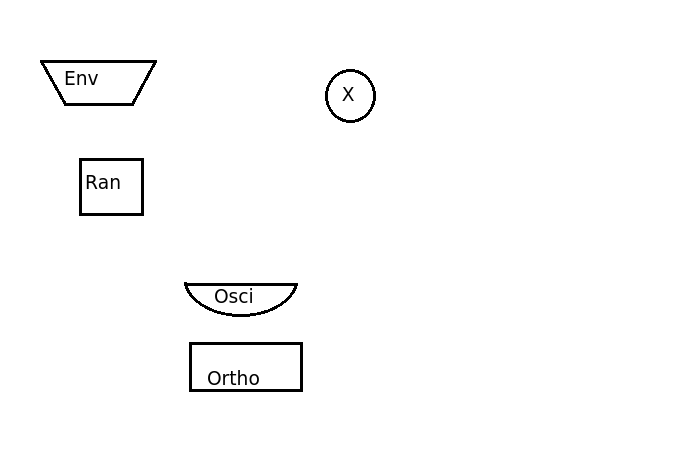
\includegraphics[scale=0.5]{./images/componentes.png}
	\caption*{}
\end{figure}

\end{frame}

\begin{frame}{Características - Arquitetura}
PROFIBUS-FMS só atende três camadas do modelo OSI (Open System Interconnection Model), Física (1), transmissão de dados (2) e Aplicação (7).

\begin{itemize}
\item O que é o modelo OSI?
\pause \item O Modelo OSI (criado em 1983 e formalizado em 1995) é um modelo de referência da ISO que tinha como principal objetivo ser um modelo standard, para protocolos de comunicação entre os mais diversos sistemas, e assim garantir a comunicação end-to-end.1

\pause \item \textbf{Esta arquitetura é um modelo que divide as redes de computadores em 7 camadas, de forma a se obter camadas de abstração}. Cada protocolo implementa uma funcionalidade assinalada a uma determinada camada.
\end{itemize}

\end{frame}


\begin{frame}{PROFIBUS - Localização na Arquitetura OSI}
\begin{figure}
	\includegraphics[scale=0.5]{./images/OSI2.png}
	\caption{Níveis da arquitetura OSI}
\end{figure}
\end{frame}

\begin{frame}{PROFIBUS - Localização na Arquitetura OSI}
\begin{figure}
	\includegraphics[scale=0.5]{./images/OSI1.jpg}
	\caption{Localização na Arquitetura OSI}
\end{figure}
\end{frame}

\begin{frame}{Camada de Aplicação}
A camada de aplicação fornece serviços de comunicação que podem ser usado pelo usuário. Sobre esta camada:
\begin{itemize}
\pause \item \textbf{A FMS (Fieldbus Message Specification) É um protocolo otimizado que oferece serviços para a comunicação de propósitos gerais}. Descreve os objetos e serviços de comunicação (serviços de mensagens com e entre dispositivos industriais programáveis como PLCs, CNs, etc. em nível de célula).
\pause \item Define um conjunto de objetos que representam recursos do dispositivo. 
\pause \item Define um conjunto de serviços de mensagens para acessar e manipular os objetos.
\pause \item Define o comportamento do dispositivo (de objetos) em frente do conjunto de serviços de mensagens.
\end{itemize}
\end{frame}

\begin{frame}{PROFIBUS FMS}
O modelo de comunicação PROFIBUS FMS possibilita: 
\begin{itemize}
\pause \item Transferência de grande quantidade de dados, por exemplo, programas, blocos de dados. 
\pause \item Integração de várias partes do processo distribuído em um processo comum usando relações de comunicação. 
\pause \item A comunicação entre as estações inteligentes.
\end{itemize}
\end{frame}

\begin{frame}{VFD – virtual Field device}
\textbf{A parte da aplicação situada no dispositivo de campo que pode ser acessada via comunicação é denominada de dispositivo virtual de campo} (VFD – virtual Field device). A figura mostra a relação entre um dispositivo real e virtual. Neste exemplo somente determinadas variáveis (isto é, número de unidades, taxa de falhas e paradas) são parte do dispositivo de campo virtual e podem ser acessadas via uma relação de comunicação. As variáveis “valor desejado” (set point) e “receita” (recipe) não estão disponíveis neste caso.

\end{frame}

\begin{frame}{VFD – virtual Field device}
\begin{figure}
	\includegraphics[scale=0.5]{./images/fieldDevice.png}
	\caption*{}
\end{figure}
\end{frame}

\begin{frame}{VFD - virtual Field device}
\begin{itemize}
\item É o objeto mais significativo do FMS. É um modelo abstrato que representa o comportamento de máquinas reais, suas características comuns respeito a sua operação externa visível desde o sistema de comunicações.

\item O objetivo deste objeto é que todos os serviços são realizados neste dispositivo virtual, e, portanto, obter uma independência de máquinas reais.
\end{itemize}
\end{frame}

\subsection{O Dicionário de Objetos}
\begin{frame}{O dicionário de objetos}
\textbf{Todos os objetos de comunicação de um dispositivo FMS são registrados em um dicionário de objetos (OD)}. O dicionário contém descrição, estrutura e tipo de dados, assim como a associação entre os endereços internos do dispositivo do objeto de comunicação e sua denominação no barramento (índice ou nome).

O dicionário de objetos se compõe dos seguintes elementos:
\begin{itemize}
\item Cabeçalho: Contém informações sobre a estrutura do OD. 
\item Lista de tipos de dados estáticos: Contém a lista de tipos de dados e estruturas de dados suportados. 
\item Dicionário de objetos estáticos: Contém a lista de objetos de comunicação estática. 
\item Lista dinâmica de variáveis: contém a lista atual de lista de variáveis conhecidas. 
\item Lista dinâmica de programas: Contém a lista de programas conhecidos.
\end{itemize}

\end{frame}

\subsection{Classificação dos Objetos}
\begin{frame}{Classificação dos Objetos}
A classificação dos objetos de comunicação se compõe em:
\begin{itemize}
\item Objetos de comunicação estática: São registrados no dicionário de objetos estáticos. \textbf{São configurados um única vez e não podem ser modificados durante a operação}. FMS reconhece cinco tipos de objetos de comunicação.
\begin{itemize}
\item Variáveis simples: Unidade indivisível.
\item Matriz (array): Série de variáveis simples do mesmo tipo.
\item Registro (record): Série de variáveis simples de diferentes tipos.
\item Domínio (domain): Área de memoria conectada logicamente. Tipo de dado sempre octeto.
\item Evento (event message): Contem uma mensagem importante.
\end{itemize}
\end{itemize}
\end{frame}

\begin{frame}{Classificação dos Objetos}
\begin{itemize}
\item Objetos de comunicação dinâmica: São registrados na seção dinâmica do dicionário de objetos. \textbf{Estes podem ser modificados durante a operação}. FMS reconhece dois tipos de objetos de comunicação dinâmicos:
\begin{itemize}
\item Chamado do programa: Os domínios são combinados em uma unidade que contém um programa executável. 

\item Lista de variáveis: Séries de variáveis simples arrays ou registros.
\end{itemize}
\end{itemize}
\end{frame}

\subsection{Endereçamento}
\begin{frame}{Endereçamento}
\begin{itemize}
\item Para acessar os objetos FMS reconhece \textbf{quatro tipos de endereçamento}, embora seu uso é limitado pelo objeto e o tipo de serviço: Endereçamento logico, endereçamento físico, endereçamento implícito e endereçamento com nomes.

\item O \textbf{endereçamento lógico é o método preferido para aceder a um determinado objeto}. O acesso é realizado com um endereço curto (índice) que é um número de 16 bits sem sinal. Cada objeto possui um único índice.

\item Objetos de comunicação podem também ser \textbf{protegidos do acesso não autorizado} através da proteção de acesso, ou os serviços de acesso é que podem ser restringidos (por ex. somente leitura).
\end{itemize}
\end{frame}

\begin{frame}{Serviçõs FMS(Confirmado e não-Confirmado)}
Os serviços FMS são um subconjunto dos serviços MMS ((MMS = Manufacturing Message Specification, ISSO 9506), que foram otimizados para aplicações de barramentos e que foram estendidos por funções para administrar os objetos de comunicação e para o gerenciamento de redes. 
\begin{itemize}
\item Os serviços confirmados podem somente ser utilizados para relação de comunicação orientada à conexão. A execução do serviço é mostrada na figura.

\item Os serviços não confirmados podem também ser utilizados em relações de comunicação sem conexão (broadcast e multicast). Podem ser transmitidos em alta ou baixa prioridade.  
\end{itemize}

Os serviços FMS são projetados especialmente para os dispositivos de fabricação, para o monitoramento e controle.

\end{frame}

\begin{frame}{Serviçõs FMS Confirmado}
\begin{figure}
	\includegraphics[scale=0.5]{./images/confirmado.png}
	\caption*{}
\end{figure}
\begin{figure}
	\includegraphics[scale=0.5]{./images/confirmado2.png}
	\caption*{}
\end{figure}
\end{frame}

\begin{frame}{Serviçõs FMS não-Confirmado}
\begin{figure}
	\includegraphics[scale=0.5]{./images/nao_confirmado.png}
	\caption*{}
\end{figure}
\end{frame}

\subsection{Grupos de Serviço}
\begin{frame}{Grupos de Serviço}
Os serviços FMS estão divididos nos seguintes grupos:
\begin{itemize}
\pause \item \textbf{Serviços gerenciamento do contexto} para estabelecer ou desligar conexões lógicas. (Initiate, Reject, abort)

\pause \item \textbf{Serviços de acesso à variáveis} utilizados para acessar variáveis, registros, matrizes ou lista de variáveis.(read, write, Physical Read, Physical Write, Information report, \ldots)

\pause \item \textbf{Serviços de gerenciamento do domínio} utilizados para transmitir, carregar e ler grandes quantidades de memória. Os dados devem ser divididos em segmentos pelo usuário.(InitiateDownloadSequence, DownloadSegment, TerminateDownloadSequence, InitiateUploadSequence, \ldots)

\end{itemize}

\end{frame}

\begin{frame}{Grupos de Serviço(continuação)}

\begin{itemize}
\item \textbf{Serviços gerenciamento de chamada de programas} utilizados para controle de programas, como compilar, iniciar e interromper programas.(CreateProgramInvocation, Start, Stop, Resume, Kill, \ldots)


\pause \item \textbf{Serviços de gerenciamento de eventos} utilizados para transmitir mensagens de alarme. Estas mensagens são enviadas como transmissões multicast ou broadcast.(EventNotification, AcknowledgeEventNotificaton, \ldots)

\pause \item \textbf{Serviços VFD Support} utilizados para identificação e status de dispositivos. Podem ser enviados espontaneamente quando requisitado por um dispositivo como transmissão multicast ou broadcast.(status, indetify e UnsolicitedStatus)
\end{itemize}
\end{frame}

\begin{frame}{Grupos de Serviço(continuação)}

\begin{itemize}
\item \textbf{Serviços de gerenciamento OD} utilizados para acessos de leitura e escrita ao dicionário de objetos. Lower Layer Interface (LLI).(get OD, Initiate put OD, Terminate put OD)

\end{itemize}
\end{frame}

\subsection{ILL: Interface Lower Layer}
\begin{frame}{A Interface da Camada Inferior ILL: Interface Lower Layer}
\begin{itemize}
\item É usada para adaptar os serviços do FMS(camada 7) com a segunda camada (transmissão de dados).

\item Incluem \textbf{tarefas de controle de fluxo e monitoração da conexão}. O usuário se comunica com outros processos através de canais lógicos denominados “associações ou relações de comunicação”. O LLI provê vários tipos de associações ou relações de comunicação para a execução do FMS e serviços de gerenciamento (FMA7). As associações de comunicação têm diferentes capacidades de conexão (isto é, monitoração, transmissão e demandas dos parceiros de comunicação). \textbf{Pode ser associações de comunicação orientadas à conexão ou sem conexão.}
\end{itemize}
\end{frame}

\begin{frame}{As associações de comunicação orientada à conexão}
\begin{itemize}

\item 
\textbf{Representam uma conexão lógica ponto-a-ponto entre dois processos de aplicação}. A conexão deve primeiro ser estabelecida com um \textbf{serviço Initiate} – iniciação antes que possa ser utilizado para transmissão de dados. Após tenha sido estabelecida com sucesso, a conexão é protegida contra acesso não autorizado e fica disponível para a transmissão de dados. 

\item
Quando a conexão não é mais necessária, ela pode ser desconectada através do \textbf{serviço Abort} - abortar. O LLI possibilita a monitoração do tempo controlado para associações de comunicação orientadas à conexão. Os atributos da conexão “aberta” e “definida” são outra importante característica de uma associação de comunicação orientada à conexão. 
\end{itemize}

\end{frame}

\begin{frame}{As associações de comunicação orientada à conexão - continuação}
\begin{itemize}
\item Nas conexões definidas o parceiro da comunicação é especificado durante a configuração. 

\item Em conexões abertas o parceiro da comunicação não especificado até a fase de estabelecimento da conexão.
\end{itemize}

\end{frame}

\begin{frame}{As associações de comunicação orientada à conexão - continuação}
\begin{itemize}
\item  FMS orientado à conexão permite a transmissão de dados de maneira cíclica ou acíclica. A transmissão de dados cíclica significa que exatamente uma variável é lida ou escrita continuamente em uma conexão. A interface fornece um método de gestão eficaz que reduz o tempo de transmissão comparado com os dados acíclicos. 
	
\item A transmissão de dados acíclica quer dizer que vários objetos de comunicação são endereçados periodicamente em uma conexão no momento que se faz à chamada do processo de aplicação.
\end{itemize}
\end{frame}

\begin{frame}{As associações de comunicação sem conexão}
Possibilita a um dispositivo comunicar-se simultaneamente com diversas estações utilizando serviços não confirmados.
\begin{itemize}
\item Em associações de comunicação broadcast, um serviço FMS não confirmado é simultaneamente enviado para todas as outras estações ligadas à rede.  
	
\item Em associações de comunicação multicast, um serviço FMS não confirmado é simultaneamente enviado para um predefinido grupo de estações.
\end{itemize}
\begin{figure}
\includegraphics[scale=0.3]{./images/associaoSemComunicacao.png}
\end{figure}
\end{frame}

\begin{frame}{As associações de comunicação sem conexão}
\begin{itemize}
\item
Todas as associações de um dispositivo FMS são registradas no CRL. Em dispositivos simples, a lista é definida pelo fabricante. No caso de dispositivos complexos, o CRL é configurável pelo usuário. 

\item
Cada associação de comunicação é endereçada por uma designação abreviada, a referência de comunicação (CREF). Do ponto de vista do barramento, uma CREF é definida pelo endereço da estação, ponto de acesso do serviço da camada dois e o ponto do acesso do LLI. O CRL contém a associação entre o CREF e os endereços da camada 2 bem como o endereço LLI. Adicionalmente, o CRL também especifica quais serviços FMS serão suportados, o tamanho dos telegramas, etc. para cada CREF.
\end{itemize}
\end{frame}

\begin{frame}{Gerenciamento de Rede}
Além dos serviços FMS, funções de gerenciamento de rede (Fieldbus MAnagement Layer 7 = FMA7) estão disponíveis. As funções FMA7 são opcionais e permitem uma configuração central. Podem ser iniciadas remota ou localmente.

\begin{itemize}
\item Gerenciamento de Contexto pode ser utilizado para estabelecer e desconectar uma conexão FMA7. 

\item Gerenciamento da Configuração pode ser usado para acessar CRL’s, variáveis, contadores estáticos e parâmetros das camadas 1/2. Pode também ser usada para identificação e registro das estações do barramento. 

\item Gerenciamento de Falha pode ser usado para indicas falhas/eventos e para reiniciar os dispositivos. 
\end{itemize}

\end{frame}

\begin{frame}{Gerenciamento de Rede(continuação)}

Um acesso uniforme para os dispositivos de configuração é obtido através da especificação da conexão de gerenciamento padrão. Uma conexão de gerenciamento padrão deve ser registrada com CREF=1 no CRL para cada dispositivo que suporte serviços FMA7 como um responder.

\end{frame}

\begin{frame}{Operação mista de PROFIBUS-FMS e PROFIBUS-DP}

\begin{itemize}
\item A operação conjunta de dispositivos FMS e DP em um barramento é uma das vantagens mais robustas de PROFIBUS. Os dois protocolos podem ser executados simultaneamente em um dispositivo. Estes dispositivos são chamados dispositivos de combinação.
 
\item A operação mista é possível porque as duas versões dos protocolos utilizam uma tecnologia de transmissão e protocolos de acesso ao barramento uniforme. As diferentes funções de aplicação estão separadas por diferentes pontos de acesso da camada 2.
\end{itemize}

\end{frame}

\begin{frame}{TRASMISSÃO CON PROFIBUS FMS}
\begin{itemize}
\item \textbf{RS 485:} É o mais utilizado pela transmissão PROFIBUS. Esta tecnologia de transmissão é conhecida como H2. A sua área de aplicação inclui todas as áreas em que é necessária alta velocidade de transmissão e facilidade de instalação.

\item \textbf{FIBRA OTICA:} Os condutores por fibra óptica podem ser utilizados para aplicações PROFIBUS em ambientes com interferências eletromagnéticas muito altas e para acrescentar a distância máxima com altas velocidades. Existem dois tipos de condutores. 
\begin{itemize}
\item Condutores de fibra óptica (plástico) para distâncias de 50m. 
\item Condutores ou fibra óptica (quartzo) para distâncias de 1 km. São muito baratos. 

\end{itemize}
\end{itemize}

\end{frame}

\begin{frame}{TRASMISSÃO CON PROFIBUS FMS - Fibra Ótica}
Muitos fabricantes oferecem conexões especiais que permitem uma conversão integrada de sinais RS 485 para trabalhar com fibras ópticas e conversão vice-versa. Isto fornece um método muito simples de intercâmbio entre transmissão RS 485 e transmissão por fibra óptica em um mesmo sistema.

\begin{table}
\begin{tabular}{|c|c|c|} \hline
& PROFIBUS FMS \\ \hline
Aplicação & Nível de célula SIMATIC S5/S7, PG/PC, HMI \\ \hline
Padrão &  EN 50 170/IEC 61158 \\ \hline
Dispositivos ligáveis & PLC, PG/PC, Dispositivos de campo \\ \hline
Tempo de resposta &  < 60 ms \\ \hline
Tamanho da rede & <= 150 km \\ \hline
Velocidade & 9.6 kbit/s -12 Mbit/s \\ \hline
\end{tabular}
\end{table}

\end{frame}

\section{Conclusão}
\begin{frame}{Conclusão}
\begin{itemize}
\item PROFIBUS FMS é um protocolo de comunicação de uso geral para supervisionamento e
controle de uma planta industrial.
\item As diversas especificações do protocolo levam em consideração a variedade
de situações encontradas no chão de fábrica.
\item O protocolo consiste em baixo nível na especificação de cabos, tensões e correntes
para instalação e comunicação dos diversos equipamentos envolvidos na automação. Em alto nível, define um conjunto de estruturas de dados para realizar o supervisionamento de forma
eficiente e segura.
\end{itemize}

\end{frame}
\end{document}
